\section{Build Encoder and Decoder in Variational AutoEncoder}

Suppose that we have a random variable $x \in \mathbb{R}^d$ and a latent variable $z \in \mathbb{R}^d$ such that ~\cite{cemgil2020autoencoding}:
\[
x \sim p(x) = \mathcal{N}(x \mid \mu, \sigma^2 \mathbf{I}),
\]
\[
z \sim p(z) = \mathcal{N}(z \mid 0, \mathbf{I}).
\]
We want to construct a Variational Autoencoder. By this, we mean that we want to build two mappings $\text{Encoder}(\cdot)$ and $\text{Decoder}(\cdot)$. The encoder will take a sample $x$ and map it to the latent variable $z$, whereas the decoder will take the latent variable $z$ and map it to the generated variable $\hat{x}$. 

If we knew what $p(x)$ is, then there is a trivial solution where:
\[
z = \frac{x - \mu}{\sigma}, \quad \hat{x} = \mu + \sigma z.
\]

In this case, the true distributions can be determined and expressed in terms of delta functions:
\[
p(x \mid z) = \delta \big(x - (\sigma z + \mu)\big),
\]
\[
p(z \mid x) = \delta \big(z - \frac{x - \mu}{\sigma}\big).
\]

\subsection{Definition of Dirac Delta Function}
\begin{itemize}
    \item The Dirac delta function  ~\cite{wheeler1997dirac} as the limit when $a \to 0$ of a sequence of normalized Gaussian distributions centered at 0 is expressed as:
    \[
    \delta_a(x) = \frac{1}{|a| \sqrt{\pi}} e^{-\left(\frac{x}{a}\right)^2}.
    \]
    \item Where:
    \begin{itemize}
        \item $a$ is the scaling parameter,
        \item $|a|$ is the absolute value of $a$,
        \item $\sqrt{\pi}$ is the normalization constant,
        \item $e^{-\left(\frac{x}{a}\right)^2}$ is the Gaussian exponential function.
    \end{itemize}
\end{itemize}

\begin{figure}[H]
    \centering
    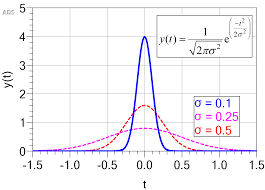
\includegraphics[width=1\linewidth]{sec/dirac.png}
    \caption{Dirac Delta Function}
\end{figure}


\subsection{Encoder and Decoder Construction}
Suppose now that we do not know $p(x)$, so we need to build an encoder and a decoder to estimate $z$ and $\hat{x}$.

\textbf{Encoder Design:}
The encoder takes the input $x$ and generates a pair of parameters $\hat{\mu}(x)$ and $\hat{\sigma}^2(x)$, denoting the parameters of a Gaussian ~\cite{zhang2015kl}. Then, we define $q_\phi(z \mid x)$ as:
\[
(\hat{\mu}(x), \hat{\sigma}^2(x)) = \text{Encoder}_\phi(x),
\]
\[
q_\phi(z \mid x) = \mathcal{N}(z \mid \hat{\mu}(x), \hat{\sigma}^2(x)\mathbf{I}).
\]

For simplicity:
\[
\hat{\mu}(x) = ax + b, \quad \hat{\sigma}^2(x) = t^2,
\]
where $a$, $b$, and $t$ are learned parameters. Substituting, we get:
\[
q_\phi(z \mid x) = \mathcal{N}(z \mid ax + b, t^2 \mathbf{I}).
\]

\textbf{Decoder Design:}
The decoder takes $z$ and reconstructs $x$ using:
\[
(\mu_e(z), \sigma_e^2(z)) = \text{Decoder}_\theta(z),
\]
\[
p_\theta(x \mid z) = \mathcal{N}(x \mid \mu_e(z), \sigma_e^2(z)\mathbf{I}).
\]

Similarly, for simplicity:
\[
\mu_e(z) = cz + v, \quad \sigma_e^2(z) = s^2,
\]
where $c$, $v$, and $s$ are learned parameters. Substituting, we get:
\[
p_\theta(x \mid z) = \mathcal{N}(x \mid cz + v, s^2 \mathbf{I}).
\]
